\documentclass[11pt, oneside]{article}   	% use "amsart" instead of "article" for AMSLaTeX format


%\usepackage{draftwatermark}
% \SetWatermarkText{Confidential}
% \SetWatermarkScale{5}
% \SetWatermarkLightness {0.85} 
% \SetWatermarkColor[rgb]{0.7,0,0}


\usepackage{geometry}                		% See geometry.pdf to learn the layout options. There are lots.
\geometry{letterpaper}                   		% ... or a4paper or a5paper or ... 
%\geometry{landscape}                		% Activate for for rotated page geometry
%\usepackage[parfill]{parskip}    		% Activate to begin paragraphs with an empty line rather than an indent
\usepackage{graphicx}				% Use pdf, png, jpg, or eps� with pdflatex; use eps in DVI mode
								% TeX will automatically convert eps --> pdf in pdflatex		
\usepackage{amssymb}
\usepackage{mathrsfs}
\usepackage{hyperref}
\usepackage{url}
\usepackage{authblk}
\usepackage{amsmath}
\usepackage{graphicx}
\usepackage{fixltx2e}
\usepackage{hyperref}
\usepackage{alltt}
\usepackage{color}


\title{Notes on Adversarial Examples}
\author{David Meyer \\ dmm@\{1-4-5.net,uoregon.edu,...\}}

% \date{}							% Activate to display a given date or no date


\begin{document}
\maketitle

\section{Introduction} 
\label{sec:intro}

\noindent
The surprising discovery of \emph{adversarial examples} by Szegedy et al. \cite{Szegedy:2013aa} has led to new ways of thinking about unsupervised training of deep models \cite{NIPS2014_5423} while at the same time casuing confusion and concern about the nature of learning in such (deep) models. These notes explore the analysis of adversarial examples given in \cite{Goodfellow:2014aa} and elsewhere.

\bigskip
\noindent
What Szegedy et al. \cite{Szegedy:2013aa}  discovered was that several machine learning models, including state-of-the-art neural networks, are vulnerable to adversarial examples. That is, these machine learning models can misclassify examples that are only slightly different (imperceptibly so in many cases)  from correctly classified examples drawn from the data distribution. In many cases, a wide variety of models with different architectures trained on different subsets of the training data misclassify the same adversarial example (this is kind of shocking). The implication is that adversarial examples expose fundamental problems in popular training algorithms.

\bigskip
\noindent
At the time of publication \cite{Szegedy:2013aa}, the cause of these adversarial examples was a mystery, and speculative explanations have suggested it is due to extreme nonlinearity of deep neural networks, perhaps combined with insufficient model averaging and insufficient regularization of the purely supervised learning problem. What \cite{Goodfellow:2014aa} shows is that these speculative hypotheses are unnecessary. As we shall see, linear behavior in high-dimensional spaces is sufficient to cause the existence of adversarial examples.  

\bigskip
\noindent
In addition, \cite{Goodfellow:2014aa} shows that generic regularization strategies such as dropout, pre-training and model averaging or ensembling  do not confer a significant reduction in a model's vulnerability to adversarial examples. On the other hand, changing to nonlinear model families such as RBF networks can confer some resistance (to such adversarial examples). These explanations reveal fundamental tradeoffs between models that are easy to train\footnote{due to their linearity} and models that use nonlinear effects to resist adversarial perturbation. Not surprisingly, these tradeoffs appear to be fundamental; however,  Goodfellow et.al. \cite{Goodfellow:2014aa} suggest that it may be possible to escape these tradeoffs by designing more powerful optimization methods that can successfully train more nonlinear models.

\section{Linear explanation of Adversarial Examples}
\label{sec:linear_explanation}
\noindent
This section follows the analysis and notation of Section 3 of \cite{Goodfellow:2014aa}, which explains the existence of adversarial examples for linear models. The section starts with a description of the precision of the sensor or storage media. Here they use the common example digital images, which often use only eight bits per pixel (gray scales) and as a result they discard all information below $\frac{1}{255}$ of the dynamic range. The point here is that since the precision of the features is limited,  it makes little sense for a classifier to respond differently to an input $\boldsymbol{x}$ than to an adversarial input $\hat{\boldsymbol{x}}  = \boldsymbol{x} + \boldsymbol{\eta}$, if of course every element of the perturbation $\boldsymbol{\eta}$ is smaller than the precision of the features. Let's say that $\epsilon$ is the largest value \emph{below} the resolution of the sensor (or storage media). Then for problems with well-separated classes, we expect a classifier to assign the same class to $\mathbf{x}$ and
$\hat{\mathbf{x}}$, so long as $||\boldsymbol{\eta}||_{\infty} <  \epsilon$ (where $||\boldsymbol{x}||_{\infty}$ is the \emph{max} or \emph{infinity} norm).

\bigskip
\noindent
Next, consider the activation induced by an adversarial example $\hat{\mathbf{x}}$:

\begin{flalign}
\hat{\mathbf{x}}  &= \mathbf{x} + \boldsymbol{\eta}   \quad \qquad \qquad \qquad  \mathbin{\#} \text{adversarial example } \hat{\mathbf{x}}  \text{ given perturbation } \boldsymbol{\eta} \\
\mathbf{w}^{\text{T}}\hat{\boldsymbol{x}}  &= \mathbf{w}^{\text{T}}\boldsymbol{x} + \mathbf{w}^{\text{T}} \boldsymbol{\eta} \qquad \qquad  \mathbin{\#} \text{activation } \mathbf{w}^{\text{T}}\hat{\boldsymbol{x}} \text{ induced by } \boldsymbol{\eta}
\end{flalign}

\bigskip
\noindent
\textbf{Notes:} 
\noindent
\begin{itemize}
\item The adversarial perturbation causes the activation to grow by $\mathbf{w}^{\text{T}} \boldsymbol{\eta}$
\item $\mathbf{w}^{\text{T}} \boldsymbol{\eta}$  is maximized, subject to $||\boldsymbol{\eta}||_{\infty} < \epsilon$, by assigning  $\boldsymbol{\eta} =  \text{sign}(\boldsymbol{w})$  \textcolor{red}{\textbf{why is this true?}}
\end{itemize}

\bigskip
\noindent
Now, if  $\dim(w) = n$ and $\overline{|w|} = m$,  then the activation $\mathbf{w}^{\text{T}} \boldsymbol{\eta}$ will grow by $\epsilon m n$  What is interesting here (among other things) is that the max norm $||\boldsymbol{\eta}||_{\infty}$, does not grow with the dimensionality of the input, while at the same time the change in activation
caused by $\boldsymbol{\eta}$ can grow linearly with $n$. As a result in high dimensional cases many very small changes to the input can add up to one large change to the output. So essentially we see that even a simple linear model can have adversarial examples if its input has sufficient dimensionality. This result is in stark contrast to thinking around the time of \cite{Szegedy:2013aa}, when it was thought that adversarial examples were a property of highly non-linear deep neural networks.

\section{What about Non-Linear Models?} 

Goodfellow, et.al \cite{Goodfellow:2014aa} hypothesizes that many neural network architectures are too linear to resist linear adversarial perturbation. These include LSTMs \cite{Hochreiter:1997aa}, ReLUs \cite{glorot2011deep} and Maxout networks \cite{goodfellow2013maxout}, which are all intentionally designed to behave in very linear ways so that they will be easier to optimize\footnote{The more nonlinear models (e.g., sigmoid networks) are carefully tuned to spend most of their time in the non-saturating, more linear regime for the same reason.}. The important conclusion here is that the behavior of simple linear models under adversarial perturbation $\boldsymbol{\eta}$ described in Section \ref{sec:linear_explanation} should also apply to ("damage") neural networks.

\begin{figure}
\center{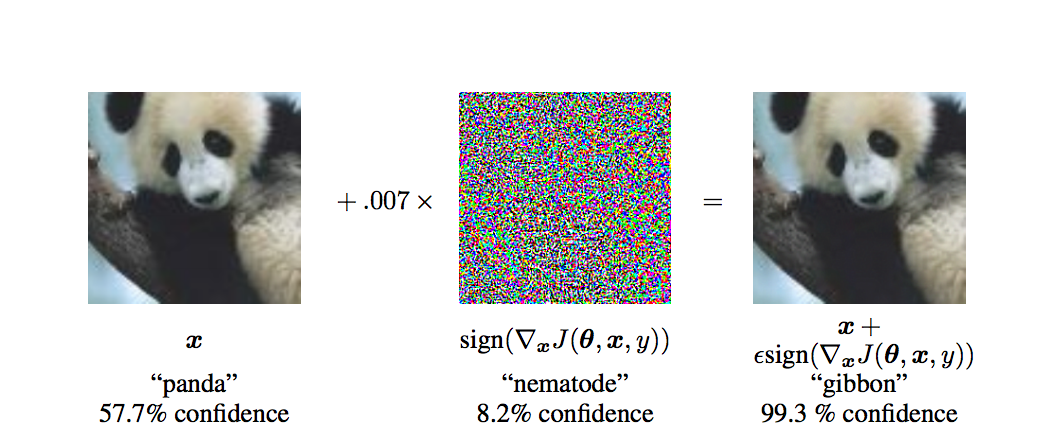
\includegraphics[scale=0.8] {images/panda.png}}
\caption{Fast adversarial example generation applied to GoogLeNet on ImageNet \cite{Szegedy:2013aa}. GoogLeNet's classification of this image can be changed, perhaps surprisingly, by adding an imperceptibly small vector whose elements are $\text{sign} (\nabla_{x}J(\boldsymbol{\theta},\textbf{x}, \textbf{y}))$, that is,  the sign of the gradient of the cost function. Here $\epsilon =.007$, roughly $2*(1/255)$,  corresponds to the magnitude of the smallest bit of an 8 bit image encoding (after GoogLeNet's conversion to real numbers).}
\label{fig:fgsm}
\end{figure}



\bigskip
\noindent
In typical form, let $\boldsymbol{\theta}$ be parameters of a model,  $\textbf{y}$ the targets associated
 with $\textbf{x}$ (in the supervised learning case) and $J(\boldsymbol{\theta},\textbf{x}, \textbf{y})$ be the cost function (optimization objective) to train the neural network.  Here we can linearize the cost function around the current value of $\boldsymbol{\theta}$, obtaining an optimal max-norm constrained perturbation of
 
 \begin{flalign}
 \label{eqn:fgsm}
 \boldsymbol{\eta} = \epsilon \text{sign} (\nabla_{x}J(\boldsymbol{\theta},\textbf{x}, \textbf{y}))
 \end{flalign}

\bigskip
\noindent
Equation \ref{eqn:fgsm} is referred to as the \emph{fast gradient sign method} for generating adversarial examples. Note that, importantly,  the gradient in Equation \ref{eqn:fgsm} can be efficiently computing using back-propagation. An example of the fast gradient sign method is shown in Figure \ref{fig:fgsm}.




\newpage
\bibliographystyle{acm}
% \bibliographystyle{plain}
\bibliography{/Users/dmm/papers/bib/ml}



\end{document} 
